\chapter{Outlook and future work}
The work presented in this document covered various thematics, all involved in the process of automatically finding new indications for approved drugs. Chapter 1 reviewed the problematic, rationale and drug repositioning efforts that have been done. Chapter 2 argued for a mathematical framework capable of capturing biomedical knowledge: I presented how description logics (DLs) can be used to achieve this task. The formalisation of the molecular machinery was implemented in Chapter 3 via the Functional Therapeutic Chemical Classification System (FTC). The resource is built by integrating information from various repositories using DLs and reasoning services. As a special care was put on scalability, the resource was successfully implemented in practice. Its content and relevance were evaluated against an existing resource, the Anatomical Therapeutic Chemical Classification System (ATC). Chapter 4 describes how the FTC can be used to perform multiple tasks, such as systematically comparing approved drugs based on their function (similarity-based approach) or identifying potential drugs from a known mode of action (MoA, via the toolbox approach). The drug repositioning hypotheses generated cover a wide range of therapeutic areas and are open for the community to investigate via a web application. With this last chapter, I wanted to communicate ideas and future projects that can be performed out of the work accomplished during my thesis and presented in this document.

Firstly, the thesis work covers only a section of the overall drug discovery process. I will present in this chapter the next logical steps and the considerations to account for while moving towards laboratory experiments. Secondly and not directly related to drug repositioning, I will introduce a follow-up analysis comparing the definition of \emph{function} from the FTC perspective against gene expression data. Thirdly and derived from the my personal experience and the theoretical work executed in Chapter 2, I will argue in favour of a simplification of biomedical knowledge representation, based on a straightforward graph structure. Finally, I will briefly describe the clinical relation between off-label use and drug repositioning and how the identification of new indications for a drug can be performed directly from hospital data.

\section{Work performed in the context of the drug discovery process}
Discovering a new active molecule includes an accurate identification of the biological mechanisms behind a disease, followed by the development of chemical compounds screened in assays and further optimised for safety and efficacy. Molecules showing some biological activity in the animal model are then finally tested in clinical trials and approved \citep{fishman2005pharmaceuticals} \citep{cooper2002optical}. The approach I presented lies in the beginning of this workflow, where the biology and chemistry are characterised, which usually takes 6 years (see Figure \ref{fig5-1}) and involves numerous experiments. Assuming I worked a maximum of 3 years on the project, I expect at least 3 more years of experimental work in order to gather enough biological evidence and validate some predictions.  The fact that the drugs investigated are all already approved should in theory facilitate further development. In practice, drug repositioning can face legal challenges (Chapter 1 section 1.1.2) regarding intellectual protection and safety in particular; therefore it should be assumed that the average time line (see Figure \ref{fig5-1}) will be respected.

\begin{figure}[ht]
    \centering
    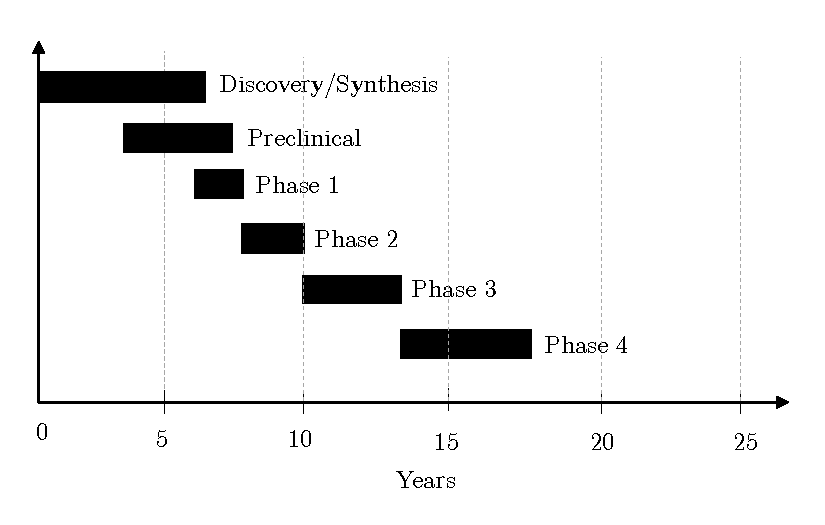
\includegraphics{fig5-1}
    \caption{Time line of the drug discovery process. My thesis work focused on the Discovery/Synthesis section of the graph.}
    \label{fig5-1}
\end{figure}

I am currently looking to set collaborations with research groups performing experiments and bioactivity assays in order to further explore the hypotheses. As many therapeutic areas are covered, priority to one disease type must be defined first. Hereof, anti-cancer agents are a good starting point. There are 84 hypotheses concerning antineoplastic compounds (\url{https://www.ebi.ac.uk/chembl/research/ftc-hypotheses/code/L01}), which gives a large enough test case. Phenotypic assays for this class of molecules are well developed and straightforward: given a line of cancer cells exposed to a chemical, they consist of measuring the ratio of cell death compared to a control \citep{garnett2012systematic}. The biological context is also better preserved than for target-based assays (Chapter 1 section 1.1.1); this format is therefore more suitable to test the hypotheses, as they have been generated while considering their physiological activities in the human body.

In summary, the work done compares and covers the initial exploration of the path towards a new therapy, which continues at this stage by performing the assays to characterise more accurately the predicted pharmacology.

\section{Comparison against functional genomics}
The FTC introduces one possible representation of the \emph{function} of approved molecules. This descriptor can be used to perform computation, as illustrated throughout this document. The Connectivity Map (Chapter 1 section 1.3.2) defines in another way the biological function of drugs, derived from gene expression experiments. As both methodologies capture the concept of \emph{function} and rely on similarity-based metrics, it would be interesting to compare the two: given a set of identical drugs, how do the similarity measures behave? Are the data in line with each other? What differences are observed? For which set of compounds? How does the definition of \emph{function} differ from a theoretical perspective (thesis) against the one derived from experimental values (CMap)? As the FTC also provides discrete categories for MoAs (toolbox approach), it could be interesting to investigate what advantage it brings when compared to gene expression data.

In this regard, I have already started to gather the data used in the work done by \cite{iorio2010discovery}. Once available, I can start the investigation and analysis of the definition of approved drugs’ functions.

\section{Biomedical knowledge: towards a simpler representation}
From a computer science perspective, ontologies are computational artefacts used to represent the knowledge of a domain of interest. The motivation behind the approach is to clarify the semantics of a vocabulary, in order to validate the consistency of a representation and derive implicit information (Chapter 2). The axioms help a computer to unambiguously interpret some knowledge. However, in practice, in the life science domain, human interpretation is always required. For instance, the content of the Gene Ontology is mostly used to perform term enrichment analysis (personal experience) or similarity based computations \citep{pesquita2009semantic}, in order to guide the interpretation of some generated data. The DLs based representation of the biomedical knowledge presented in Chapter 2 can be arguably seen as heavy and too complicated for the results sought. The axioms present in the FTC are based on existential restriction patterns in order to logically link concepts via an object property. This representation could be simplified by considering all concepts as instances directly linked by a property (section 2.3.3.2) and resulting in a graph. This model is close to the one proposed by the Resource Description Framework (RDF), part of the semantic web’s specifications \citep{klyne2006resource}. The ambiguity between instances and concepts is known as punning and is allowed by the Web Ontology Language; it is widely used in the RDF representation of biomedical databases such as ChEMBL or Uniprot \citep{jupp2014ebi}, as it allows for the straightforward representation of the required information.

Considering this, the future work I will do on biomedical knowledge representation will go in this direction: representing life science knowledge as a simple graph while keeping the expressivity of roles. I expressed most of the FTC semantics using roles, which are highly interoperable one with another (cf section 3.2.9.2). As far as I know, there exists no framework within the semantic web specification stack (RDF, RDFS, OWL and related profiles) allowing the extended use of object properties or role axioms (transitivity, chained property) in combination with a simple graph representation like the one featured by RDF. With such a language, it would be possible to keep the advantages of scalable reasoning (subset of \dl{EL\textsuperscript{++}}) while considerably simplifying the initial representation and discarding cumbersome axioms not so helpful for biological interpretation later on, for instance existential restrictions.

This language will lie between network biology \citep{ravasz2002hierarchical}, semantic nets \citep{schubert1978structure}, Petri Nets \citep{murata1989petri}, pathways databases \citep{schaefer2009pid} and RDF while keeping the important reasoning services. The added value on the top of these previous approaches will reside in the importance given to the edges between nodes, in particular their biomedical semantics and what can be derived and expanded from them. The black box machine analogy is still valid for this representation, and the implementation can be done in many other ways than the one presented with the FTC. The focus of the language would be the deductions that can be derived from it rather than maximizing interoperability between resources. A graph representation also allows full control of data querying and analysis; it would also be easier to derive metrics such as similarity values, commonly used in biology \citep{stevens2007using}. Moreover, some robust solutions are available at the time of writing \citep{have2013graph}.

More work has to be done in order to fully express the idea, but it can be summarised as a simple and customisable graph-based framework to locally integrate biomedical information, with a strong focus on edges semantics interoperability (\emph{part-of}, \emph{regulates}, \emph{involved-in} combined with rules).

\section{Off-label uses and clinical drug repositioning}
In the context of my work, I came to discuss drug repositioning with some physicians practising in a hospital (Addenbrooke's - Cambridge UK). After the meetings and analyses presented in Chapter 4 (section 4.3.1), it clearly appeared that drug repositioning relates closely to off-label prescriptions. In practice, doctors indicate a treatment for a different usage than what it is regulated for 20 percent of the time. \citep{cras2007off}. Sometimes a new pharmacological effect is identified \citep{stephens2009dark}, and the indication line of the drug can be expanded accordingly. This type of evidence is very valuable, as it reflects the effect of the drug directly in human population. A meticulous recording and automated analysis can help to identify such cases rapidly. Off-label prescription data is currently not recorded in all hospitals (personal discussion with physicians), and a computer system handling it might be a smart way to directly capture relevant hypotheses. It could be developed on the top of an electronic medical records system \citep{cras2007off} or as a stand-alone application. I am currently investigating what would be the requirements of such a workflow, in collaboration with physicians and biomedical researchers.

\hrulefill

This chapter concludes the thesis work I decided to present in more details. The reader can refer to the Appendices in order to find the full list of the peer-reviewed articles I contributed to and published in the course of the doctorate, as a complementary source of information (\cite{croset2013brain}, \cite{croset2013functional}, \cite{croset2010calbc}, \cite{croset2011exploring}, \cite{rebholz2013case}, \cite{yan2012finding}, \cite{herrero2013ontology}, \cite{croset2013brain2}, \cite{croset2012integration}).

I hope to have presented clearly and concisely the message I wanted to communicate: living organisms, just as machines, are subject to dysfunction, which can be investigated for repair using description logics. The source of this document is free, open and available online at \url{https://github.com/loopasam/thesis}.
